\chapter{}{{Multi-Model Approaches to Solar Forecasting}}{Multi-Model Blending Approaches to Solar Irradiance Forecasting}

\subchapter{Overview}
\par There is a significant variability in the \textit{global horizontal irradiance} (GHI) measured by NWP models with respect to cloud conditions. Mathiesan and Kliessl \cite{multimodel_overpredict} found that the NAM Forecast System tends to overpredict GHI in clear-sky conditions, i.e. sky conditions in which visible clouds are absent, by up to 40 percent. They proposed a bias-correction scheme to selectively correct the overpredicted GHI. In this scheme, they derived a multivariate fourth-order model-output statistics (MOS) correction function depending on solar zenith angle ($\theta_z$) and clear-sky index ($K_c$). Based on $K_c$, sky-conditions for the forecasts were determined. The bias correction function was employed on the forecasts possessing a positive bias in clear-sky conditions. 

\par However, Diagne et al. \cite{litrev_nwp5} noted that this bias-correction methodology was not adequate, as even the accurate forecasts were unnecessarily corrected. Thus, a need for a superior bias-correction methodology depending on cloud-conditions was identified, so as to improve the GHI predicted by the NAM Forecast System. The experiments conducted in this chapter are devoted towards exploring theory-driven approaches for this purpose.

\par There are multiple empirical solar radiation formulations which have been extensively discussed in literature \cite{litrev_pvlib10}\cite{litrev_pvlib11}\cite{litrev_pvlib12}\cite{litrev_pvlib13}\cite{litrev_pvlib14}\cite{litrev_pvlib9}, which compute the different components of solar irradiance from environmental conditions, through experimental observations. These can be broadly classified into \textit{decomposition} and \textit{parametric} models \cite{litrev_pvlib3}. Using assumptions on solar geometry and transmittance, the former are used to estimate direct beam and diffuse irradiance. The latter are useful for approximating daily solar radiation reaching tilted surfaces. In this chapter, two such empirical solar radiation models, \textit{Clear-Sky Scaling} and \textit{Liu-Jordan Model} are discussed, which help estimate different components of global solar radiation, including GHI.

\restoregeometry\noindent
\par In climatic research, in order to be able to distinguish between clear-sky and cloudy-sky conditions effectively, measures such as \textit{clear-sky index} ($K_c$) and \textit{clearness index} ($K_t$) have been introduced. Clear-sky index is generally described as the ratio of measured global horizontal irradiance in a system to its measure in clear-sky conditions, estimated with the help of a clear-sky solar radiation model. It makes accurate and continuous determination of cloud amount from surface measurements possible \cite{multimodel_clearskyindex}. In contrast, clearness index is simply a ratio of the measured irradiance at a location, to the extraterrestrial irradiance calculated at the location. It is extremely useful as it incorporates both light scattering and light absorption, which is beneficial towards estimating the shortwave radiation reaching the surface of the earth.

\par In this work, a theory-driven multi-model blending approach is explored towards correcting the reported bias in GHI. This is done by combining the NAM Forecast System with the empirical \textit{Clear-Sky Scaling} technique based on $K_c$ estimates, and with the \textit{Liu-Jordan} model based on $K_t$ estimates. In the case of the former, the clear-sky Ineichen Model was used to compute the clear-sky GHI, which goes into estimating $K_c$. From among the 00h, 06h, 12h, 18h UTC forecasts released by the NAM Forecast System, 18h NAM forecasts with $K_c > 0.85$ were corrected, by substituting the GHI from NAM Forecast System ($GHI\textsubscript{NAM}$) with the arithmetic mean of the $GHI\textsubscript{NAM}$ and GHI estimates from \textit{Clear-Sky Scaling} technique ($GHI\textsubscript{CS}$). 

\par Predictive models implementing the random forest technique were developed utilizing $GHI\textsubscript{NAM}$ and $GHI\textsubscript{CS}$ independently. The models were compared, and it was observed that such a bias-correction scheme led to an improvement in performance, reducing the mean absolute error ($MAE$) by 4.95\%, 4.53\% and 4.12\% for the dual-axis tracking, fixed-axis and single-axis tracking solar arrays respectively. A similar comparison was performed by including other weather variables from NAM Forecast System, and incorporating the input-selection scheme described in 3.2. However, in this case, the model-blending approach did not lead to an improvement in performance, resulting in an $MAE$ of 72.57 $W/m^2$, 44.91 $W/m^2$ and 63.6 $W/m^2$ for each of the solar arrays.

\par A similar model-blending approach was evaluated for combining the NAM Forecast System with \textit{Liu-Jordan} model, depending on $K_t$ estimates. $K_t$ was computed based on estimations for \textit{extraterrestrial radiation} and \textit{solar zenith angle} for the target location, i.e. Athens, Georgia. For the 18h NAM forecasts with $K_t > 0.35$, $GHI\textsubscript{NAM}$ was substituted with the arithmetic mean of $GHI\textsubscript{NAM}$ and GHI from \textit{Liu-Jordan} model ($GHI\textsubscript{LJ}$). Predictive models implementing the random forests technique were developed, utilizing $GHI\textsubscript{NAM}$ and $GHI\textsubscript{LJ}$ independently as well. It was observed that the former performed better, with the $MAE$ improving by 4.17\%, 4.14\% and 3.62\% for dual-axis tracking, fixed-axis and single-axis tracking solar arrays respectively. Additionally, predictive models implementing random forests technique were developed by including other weather variables from NAM Forecast System, and incorporating the input-selection scheme. For these models, the model-blending technique \textit{slightly deteriorated} the performance, resulting in an $MAE$ of 72.74 $W/m^2$, 45.25 $W/m^2$ and 63.97 $W/m^2$ for each of the solar arrays.

\par In order to study the utility of clear-sky index, another model-blending methodology was explored in which clear-sky index was included as a predictor variable to various machine learning models rather than GHI. The intuition behind this approach was to capture the diurnal and seasonal cyclicity capturing ability of this measure \cite{multimodel_clearskyindex2}. Such an ability can be attributed to the \textit{solar zenith angle}, which goes into the computation of this measure and helps track the position of the Sun. An input-selection scheme in line with that followed in Chapter 3 was used to generate a weather forecast data for the machine learning models, so as to forecast solar irradiance for the dual-axis tracking, fixed-axis and single-axis tracking solar arrays.

\par The performance of such predictive models was worse than that obtained by utilizing the input-selected weather forecast data from the NAM Forecast System (reported in Tables~\ref{Tab:fs_array_a}, \ref{Tab:fs_array_b}, \ref{Tab:fs_array_e}). The $MAE$ increased for the best performing \textit{random forests} by 11.59\%, 9.8\% and 9.42\% along each of the solar arrays, recording an $MAE$ of 79.58 $W/m^2$, 49.18 $W/m^2$ and 69.98 $W/m^2$ respectively. A stratified diurnal and seasonal analysis was performed on the predictions attained through this methodology. The presumed cyclicity-capturing ability of the clear-sky index measure did not translate into improving the performance of the predictive models across corresponding seasons.

\subchapter{Empirical Solar Radiation Models}
\par Solar researchers have developed various formulations through experimental observations, which help in determining the relation between different components of solar radiation and various meteorological parameters. Of these, \textit{parametric} models require information about atmospheric conditions such as turbidity, cloud cover, etc. to be able to formulate the different components of solar irradiance such as diffuse horizontal irradiance (DHI), direct normal irradiance (DNI) and global horizontal irradiance (GHI). \textit{Decomposition} models formulate equations to estimate the solar irradiance components based on the correlations between them. Such formulations are relevant, especially in cases where meteorological data is not adequately available.

\par DHI is the amount of solar radiation received by a horizontal surface, which has been scattered by the molecules and particles in the atmosphere. It is the part of solar radiation which does not belong to the $5^{\circ}$ field of view concentric around the sun. DNI is the direct radiation received on a plane normal to the sun over the total solar spectrum. It is an essential component of global irradiance, especially in cloudless conditions. GHI is the total amount of such terrestrial irradiance which is received by a surface horizontal to the surface of the earth. It can measured with the help of pyranometers, and in general, can be computed from DHI and DNI using the following equation, where $\theta_z$ is the \textit{solar zenith angle} (the angle between sun and the vertical):
\begin{equation}\label{eq:ghi}
    GHI = DHI + DNI . cos(\theta_z)
\end{equation}

\par Holmgrem et al \cite{pvlib_Holmgren2018} contributed to building \textit{pvlib-python}\footnote{\url{https://github.com/pvlib/pvlib-python}} an open source, python-based software, ported from the PVLIB MATLAB toolbox developed at Sandia National Laboratories. This software provides a set of utilities for simulating the performance of the photovoltaic energy systems, with implementations of algorithms related to solar energy. Specifically, it contains components to obtain weather forecast data from NOAA/NCEP/NWS models including the GFS, NAM, RAP, HRRR, and the NDFD, retrieved from the UNIDATA THREDDS servers; and components to convert this weather forecast data into a PV power forecast.

\par For our experiments, we retrieved a NAM data product ($NAM\textsubscript{awphys}$) from the NCEP servers. This is different from the one retrieved by \textit{pvlib-python} ($NAM\textsubscript{awip}$) in that the former is a full complement of both the pressure level fields and surface-based fields, while the latter is a full complement of just the surface-based fields. To be able to extend the solar energy related algorithms to the NAM weather forecast data collected by us, making it compatible with $NAM\textsubscript{awip}$ becomes essential.

\par $NAM\textsubscript{awip}$ data retrieved by \textit{pvlib-python} consists of the following surface-level parameters: air temperature, wind speed, total clouds, low clouds, mid clouds and high clouds. In order to enable the use of \textit{pvlib-python} functionalities on the weather forecast dataset collected by us, equivalent surface-level fields were identified in $NAM\textsubscript{awphys}$. In this work, each of the irradiance metrics GHI, DHI and DNI were computed from the \textit{pvlib-python} compatible NAM dataset using two empirical solar radiation models implemented in the software: Clear-sky Scaling, Liu-Jordan Model.
\vspace{0.3cm}

\subsubchapter{Clear-sky Scaling}
\par Global horizontal irradiance can be measured with the help of a pyranometer on a horizontal surface. For this reason, it is typically the most common type of irradiance measurement. Knowledge of clear sky conditions, i.e. where the visible clouds are absent, is a key requirement for forecasting terrestrial solar radiation. Empirical solar radiation models such as clear-sky models estimate the solar radiation under a cloudless sky based on various atmospheric parameters. Such models can generally be validated by comparing the estimated irradiance with the measured irradiance in clear-sky conditions. 

\par Several parametric models have been proposed in literature to compute the different components of solar radiation from environmental conditions such as atmospheric turbidity, fractional sunshine, perceptible water vapor, etc. Ineichen et al \cite{pvlib_ineichen} formulated a model to compute Linke turbidity independent of the airmass, and clear-sky GHI from this metric. In this technique, the \textit{Ineichen Clear-Sky Model} was used to compute the clear-sky GHI ($GHI\textsubscript{CS}$). Going by Larson et al's \cite{pvlib_larson} work, this was scaled on the basis of the total cloud cover ($TCC$) according to the following equation: 
\begin{equation}\label{eq:ghi_cs}
    GHI = GHI_{CS} . [0.35 + 0.65(1 - TCC)]
\end{equation}

\par In addition, the popular \textit{Direct Insolation Simulation Code} (DISC) model introduced by Maxwell et al. \cite{pvlib_disc} was used to compute the direct beam component of global solar radiation, i.e. DNI. The diffuse part of global solar radiation, i.e. DHI was computed by subjecting the GHI (estimated with Eq.~\ref{eq:ghi_cs}) and DHI to Eq.~\ref{eq:ghi}

%\par Maxwell et al \cite{pvlib_disc} introduced the popular \textit{Direct Insolation Simulation Code} (DISC) model to compute cloudy-sky DNI from GHI (in this case, computed with Eq. \ref{eq:ghi_cs}) and other environmental factors. Clearness index is the fraction of the solar radiation transmitted through the atmosphere to strike the earth's surface. DISC model uses empirical relationships between the direct and global components of this measure to estimate the direct beam component. Additionally, the clear-sky DHI component can be evaluated from these irradiance metrics and the solar zenith angle using the equation described in Eq. \ref{eq:ghi}.

\subsubchapter{Liu-Jordan Model}
\par Decomposition models typically utilize only data pertaining to global solar radiation, to estimate the diffused component. They depend on the atmospheric effects in an isolated place, varying according to time of the year, season and climatic conditions \cite{pvlib_liujordan}. Liu et al. proposed one of the simplest and earliest models of radiation, the Liu-Jordan model \cite{pvlib_liujordan2}, which presumes that diffuse radiation intensity is distributed uniformly over the whole sky. In this model, the diffuse irradiance on a surface tilted towards the equator at an angle $\theta$, where $I_D$ is the diffuse radiation on a horizontal surface is given by the following empirical equation:

\begin{equation}\label{eq:lj_dhi}
    I_{Dt} = I_D . (\frac{1 + cos\theta}{2})
\end{equation}

Liu-Jordan model, though simple, is one of the more accurate models for estimating diffuse radiation on inclined surfaces \cite{pvlib_liujordan3}. This model helps determine DNI, GHI from properties such as extraterrestrial flux, transmittance, and optical air mass number. It has been observed that the Liu-Jordan model provides a good fit to empirical data under overcast skies, but underestimates the solar radiation on tilted surfaces when used for partially-clear and clear-sky days \cite{pvlib_liujordan4}.

\subchapter{Experiment Setup}
\par In this chapter, two series of experiments are performed towards predicting solar irradiance on each of the dual-axis tracking, fixed-axis and single-axis tracking solar arrays. They can be summarized as follows:
\setlist{nolistsep}
\begin{itemize}[noitemsep]
    \item contrasting the utilization of GHI (from NAM Forecast System), adjusted GHI (from blending NAM Forecast System with \textit{Clear-Sky Scaling} and \textit{Liu-Jordan} techniques) as a predictor variable
    \begin{enumerate}[label=(\alph*)]
        \item comparing performance of \textit{random forests} utilizing GHI and adjusted GHI independently as predictors
        \item comparing performance of \textit{random forests} utilizing other input-selected NAM weather variables along with GHI and adjusted GHI as predictors
    \end{enumerate}
    \item contrasting performance of predictive models utilizing \textit{clear-sky index} rather than GHI
\end{itemize}


\par In the first series of experiments, a theory-driven bias-correction scheme combining the NAM Forecast System with empirical solar radiation models such as \textit{Clear-Sky Scaling} and \textit{Liu-Jordan} is explored. In Chapter 3, it was observed that the \textit{random forest} was the best performing machine learning model for the purpose of solar irradiance forecasting. Independent predictive models were developed using this algorithm, utilizing GHI estimates from NAM Forecast System and bias-corrected GHI estimates from model-blending as input. These models were compared and analyzed, so as to gauge the effect of the model-blending scheme. In order to enable a consistent comparison of model performance, evaluation metrics used in Chapter 3, i.e. mean absolute error ($MAE$) and coefficient of determination ($R^2$) were used in this chapter as well. 

\begin{figure}[ht]
    \begin{center}
    	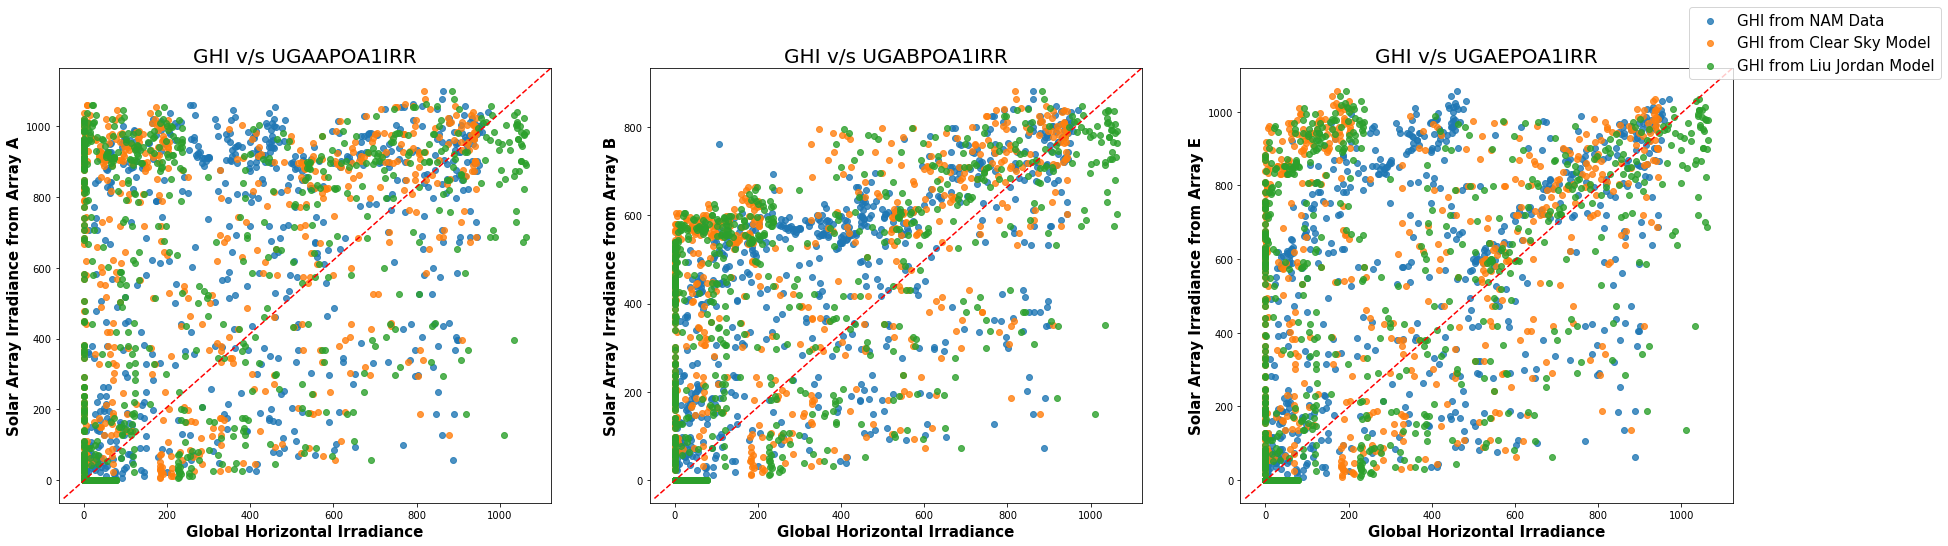
\includegraphics[width=\textwidth]{chapter4/fig_ghi_irradiance.png}
    	\caption[GHI from NAM data, Clear-sky Scaling and Liu-Jordan against irradiance observations from dual-axis tracking, fixed-axis, single-axis tracking solar arrays through 2017.]{Correlation of the first feature projection corresponding to GHI from NAM data, Clear-sky Scaling and Liu-Jordan Model, with respect to irradiance observations from dual-axis tracking (left), fixed-axis (center) and single-axis tracking (right) solar arrays through 2017.}
    	\label{fig:fig_ghi_irradiance}
    \end{center}
\end{figure}

\par Furthermore, other NAM weather variables such as air temperature, height at planetary boundary layer, and total cloud cover, which were observed to be effective for solar irradiance prediction were also considered. 
Predictive models were developed by including these weather variables along with the different variants of GHI described earlier. This weather forecast dataset was input to \textit{random forests} with the input-selection scheme described in 3.2, so as to predict solar irradiance on each of the solar arrays. The performance of these predictive models was compared with models utilizing input-selected NAM weather forecast data, in which the GHI estimates weren't adjusted. 

\par A second series of experiments was performed, where multiple machine learning models were developed using \textit{clear-sky index} rather than GHI, along with the other NAM weather variables. An input-select scheme in line with that in 3.2 was designed to selectively pick relevant feature projections of the weather variables in the forecast horizon. Solar irradiance predictions were made utilizing this weather forecast data on each of the dual-axis tracking, fixed-axis and single-axis tracking solar arrays. A stratified diurnal and seasonal analysis of the performance of these predictive models was performed, to gauge the cyclicity-capturing ability of these models.

\subsubchapter{Blending NAM Forecast System with Empirical Models}
\par \textit{Clear-Sky Scaling} and \textit{Liu-Jordan} techniques were used to evaluate GHI ($GHI\textsubscript{CS}$ and $GHI\textsubscript{LJ}$ respectively) from the meteorological variables in the NAM Forecast System. Both of these GHI estimates were compared with the GHI from the NAM Forecast System ($GHI\textsubscript{NAM}$) for each of the 00h, 06h, 12h and 18h NAM forecasts. In Fig.~\ref{fig:fig_ghi_comparison}, the residuals of the first feature projection of $GHI\textsubscript{CS}$ and $GHI\textsubscript{NAM}$ (left), $GHI\textsubscript{LJ}$ and $GHI\textsubscript{NAM}$ (right) with respect to the corresponding irradiance observations from the fixed-axis solar array were plotted for all NAM forecasts in 2017. 

\par Residuals correspond to the difference between the target irradiance observations and the modeled GHI estimates. Thus, in Fig.~\ref{fig:fig_ghi_comparison}, lying above the X-axis signifies the under-estimation of the corresponding GHI values, and lying under the X-axis signifies the over-estimation of corresponding GHI values. For both the 00h and 06h NAM forecasts, the residuals in both the sub-plots are mostly close to the X-axis, except for a small period for the 00h NAM forecasts. The 00h NAM forecasts correspond to late-evening at the target location. The period for which the residuals corresponding to $GHI\textsubscript{CS}$ and $GHI\textsubscript{LJ}$ are under the X-axis signifies the middle of the year where days are longer, thus leading to possible over-estimation of GHI by the empirical techniques. Meanwhile, the 06h NAM forecasts correspond to night-time at the target location, where there is no sun. Thus, the near-zero residual values for these forecasts are justified. 

\par The residuals of GHI estimates from 12h NAM forecasts are consistently above the X-axis, with those corresponding to the GHI estimates from \textit{Clear-Sky Scaling} and \textit{Liu-Jordan} techniques being constantly greater than the residuals corresponding to the GHI estimates from the NAM Forecast System. This illustrates the under-prediction of GHI by all the modeling techniques, with that from the empirical techniques being greater than the NAM Forecast System. Similarly, residuals corresponding to 18h NAM forecasts are studied as well. However in this case, more variability of the GHI estimates was observed, with a considerable number of over-predicted GHI estimates across all the modeling techniques. 


\begin{figure}
\begin{center}
    \subfloat[NAM Forecast System + Clear-Sky Scaling]{
        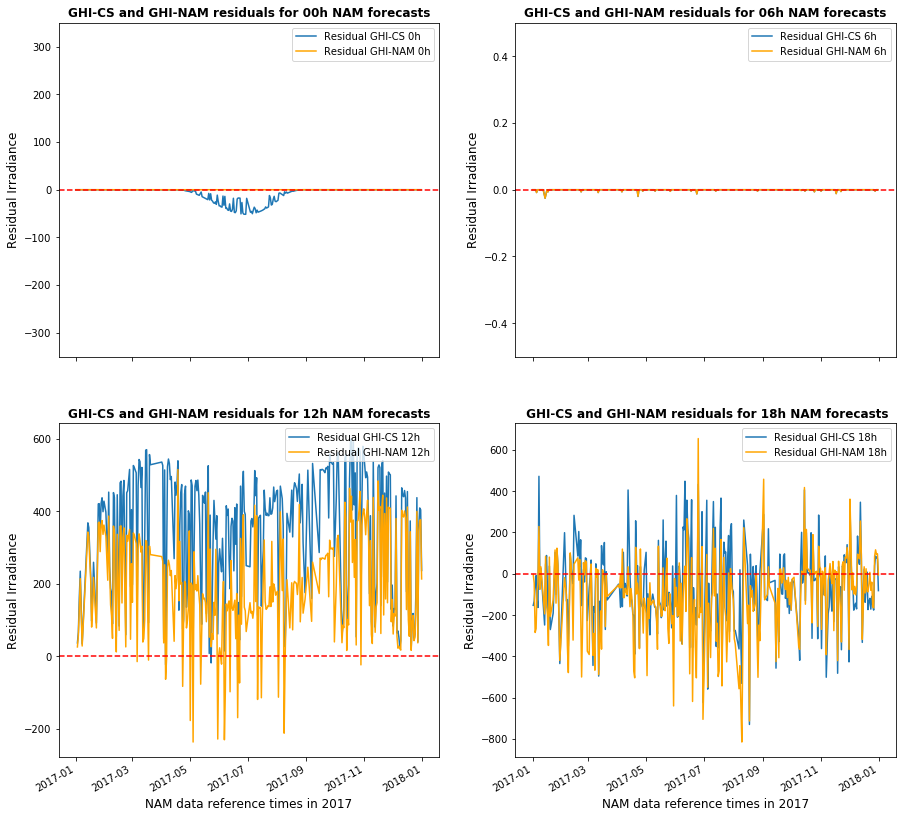
\includegraphics[width=0.46\textwidth]{chapter4/fig_ghi_comparison_cs.png}
        }
    \hspace{5mm}
    \subfloat[NAM Forecast Sytem + Liu Jordan Model]{
        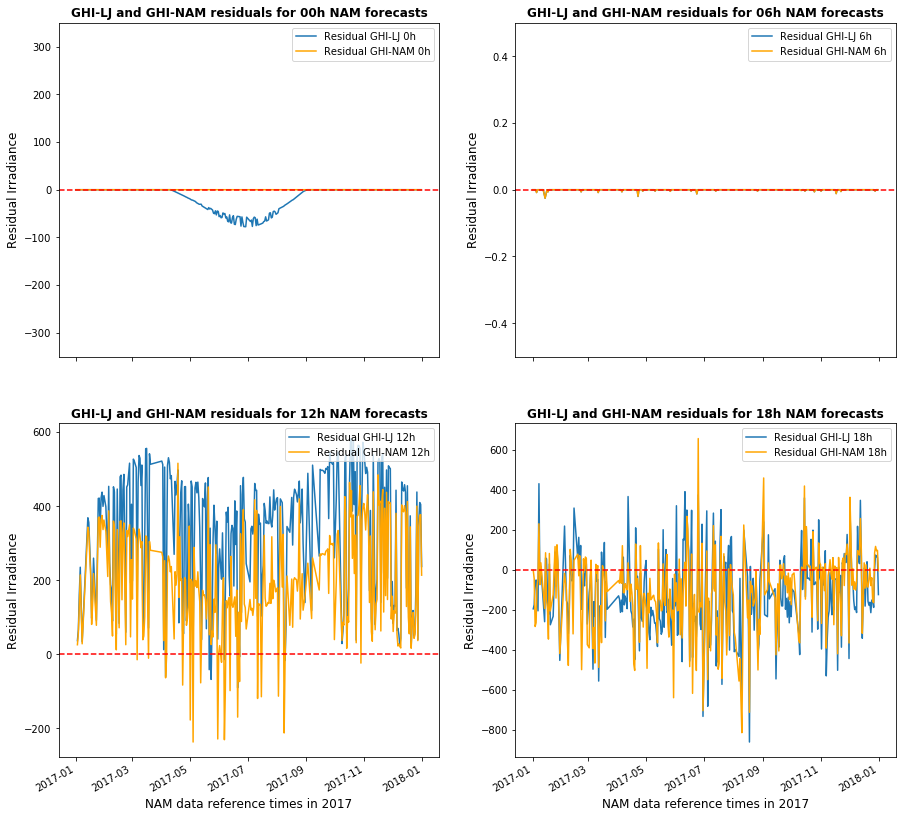
\includegraphics[width=0.46\textwidth]{chapter4/fig_ghi_comparison_lj.png}
        }
    \caption[Comparing GHI estimates from Clearsky-Scaling ($GHI\textsubscript{CS}$) and Liu-Jordan ($GHI\textsubscript{LJ}$ techniques with NAM Forecast System ($GHI\textsubscript{NAM}$ for 00h, 06h, 12h, 18h NAM forecasts]{Comparing GHI estimates from Clearsky-Scaling ($GHI\textsubscript{CS}$) and Liu-Jordan ($GHI\textsubscript{LJ}$ techniques with NAM Forecast System ($GHI\textsubscript{NAM}$ for 00h, 06h, 12h, 18h NAM forecasts: Residuals of $GHI\textsubscript{CS}$ (blue) and $GHI\textsubscript{NAM}$ (orange) with respect to fixed-axis solar array irradiance observations for individual weather forecasts in 2017 (left); Residuals of $GHI\textsubscript{LJ}$ (blue) and $GHI\textsubscript{NAM}$ (orange) with respect to fixed-axis solar array irradiance observations for individual weather forecasts in 2017 (right).}
    \label{fig:fig_ghi_comparison}
\end{center}
\end{figure}

\par To be able to explain the variability in the GHI estimates of the 18h NAM forecasts better, studying measures which determine the amount of cloudiness in the sky is essential. In this regard, \textit{clear-sky index} and \textit{clearness index} were explored. Clear-sky index helps in the removal of diurnal and seasonal signals from a given set of radiation data \cite{expt_clearsky_index}. This can be attributed to the fact that the \textit{solar zenith angle}, i.e. the elevation angle of the Sun is utilized in the estimation of this measure. In contrast, \textit{Clearness index} helps in estimating the clearness in the sky and can be determined for a specific day based on collected meteorological data and knowledge of extraterrestrial irradiance. It is extremely important in the parameterization of \textit{Liu-Jordan} model. 

\par The \textit{Ineichen Model} was used to compute the clear-sky GHI, which goes into the estimation of \textit{clear-sky index}. For the computation of clearness index, estimation of extraterrestrial radiation for a day of the year, and the estimation of solar zenith angle are necessary. Reda et al. \cite{multimodel_spa} proposed \textit{Solar Position Algorithm}, an implementation of which was used in the determination of the solar zenith angle. The extraterrestrial radiation was determined using an implementation of the algorithm described by Spencer. J in \cite{multimodel_extraterrestrial}. Both of these measures were formulated such that the negative and non-finite values are truncated to zero, and the maximum value is 2, allowing the over-irradiance events typically seen in sub-hourly data. In Fig.~\ref{fig:fig_kc_kt_18h}, to further study the variability in $GHI\textsubscript{CS}$ and $GHI\textsubscript{LJ}$, clear-sky index and clearness index were plotted for the 18h NAM forecasts.

\begin{figure}
\begin{center}
    \subfloat[]{
        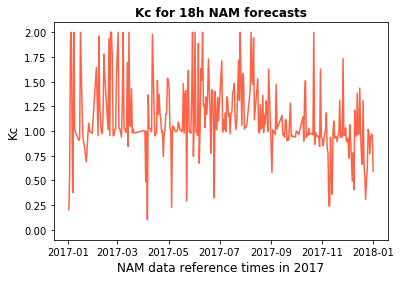
\includegraphics[width=0.46\textwidth]{chapter4/fig_kc_18h.png}
        }
    \hspace{5mm}
    \subfloat[]{
        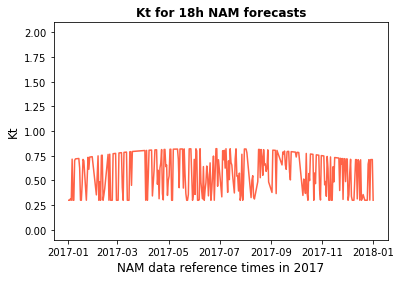
\includegraphics[width=0.46\textwidth]{chapter4/fig_kt_18h.png}
        }
    \caption[Clear-Sky Index and Clearness Index estimates for 18h NAM forecasts in 2017]{Clear-Sky Index ($K_c$, left) estimates and Clearness Index ($K_t$, right) estimates for 18h NAM forecasts in 2017.}
    \label{fig:fig_kc_kt_18h}
\end{center}
\end{figure}

\par Generally, clear-sky index values greater than 1 indicate higher solar irradiance observations. It was observed that the clear-sky index for the 18h NAM forecasts were highly variable, and identifying clear-sky periods based on the clear-sky index was not as straightforward. Thus, a randomized cross-validated grid search was performed to find a threshold for the clear-sky index, above which clear-sky periods could be presumed, and $GHI\textsubscript{NAM}$ could be corrected. The proposed bias-correction involved substituting $GHI\textsubscript{NAM}$ with the arithmetic mean of $GHI\textsubscript{NAM}$ and $GHI\textsubscript{CS}$. Based on such an approach, it was found that $K_c$ could be thresholded at 0.85. For the sake of convenience, in this work, the GHI estimates corresponding to the model-blending techniques will be referred to as \textit{adjusted GHI}, and those corresponding to model-blending between the NAM Forecast System and \textit{Clear-Sky Scaling} as \textit{adjusted} $GHI\textsubscript{NAM+CS}$.

\par A similar randomized cross-validated grid search was performed to identify a threshold for the clearness index as well. For NAM forecasts with clearness index greater than this threshold, sunny conditions could be presumed, and below which, cloudy sky conditions could be presumed. Such a threshold was identified at 0.35. Thus, for all 18h NAM forecasts with $K_t > 0.35$ (i.e. possessing sunny sky conditions), $GHI\textsubscript{NAM}$ was adjusted by substituting it with the arithmetic mean of $GHI\textsubscript{NAM}$ and $GHI\textsubscript{LJ}$. For the sake of convenience, such bias-corrected GHI estimates will be referred to as \textit{adjusted} $GHI\textsubscript{NAM+LJ}$.

\par \textit{Random forests} were the better performing machine learning models for solar irradiance prediction in Chapter 3. Separate predictive models were developed using this algorithm, utilizing $GHI\textsubscript{NAM}$, \textit{adjusted} $GHI\textsubscript{NAM+CS}$ and \textit{adjusted} $GHI\textsubscript{NAM+LJ}$ alone. The performance of each of these models forecasting solar irradiance on the dual-axis tracking, fixed-axis and single-axis tracking solar arrays was compared.

\par In addition, such predictive models were also developed by including additional NAM weather variables along with $GHI\textsubscript{NAM}$, \textit{adjusted} $GHI\textsubscript{NAM+CS}$ and \textit{adjusted} $GHI\textsubscript{NAM+LJ}$ respectively. Relevant feature projections were chosen for each of them based on the input-selection scheme described in 3.2. \textit{Liu-Jordan} model has been shown to be effective in predicting diffuse irradiance on inclined surfaces. This was also verified as the DHI estimated by this technique was highly correlated with ground-based solar irradiance observations. Thus, DHI estimated by \textit{Liu-Jordan} model was included as a predictor to the models involving \textit{adjusted} $GHI\textsubscript{NAM+LJ}$. Performance of models using these three variants of weather forecast data was compared for the dual-axis tracking, fixed-axis and single-axis tracking solar arrays.
\clearpage

\subsubchapter{Predictive Modeling Using Clear-Sky Index}
\par For each of the 25 GHI feature projections in the NAM Forecast System, corresponding clear-sky GHI estimates were computed using the \textit{Ineichen Clear-Sky Model}. These estimates were used to determine the clear-sky index ($K_c$) values, resulting in 25 feature projections for this measure. A higher dependency was observed between $K_c$ and solar irradiance observations from the solar farm, as compared to the other NAM weather variables. Thus, following the input-selection scheme described in 3.2, a mutual information matrix was computed for each of the feature projections of $K_c$ with respect to the solar irradiance observations from fixed-axis solar array in the forecast horizon.

\begin{figure}[htb]
    \begin{center}
    	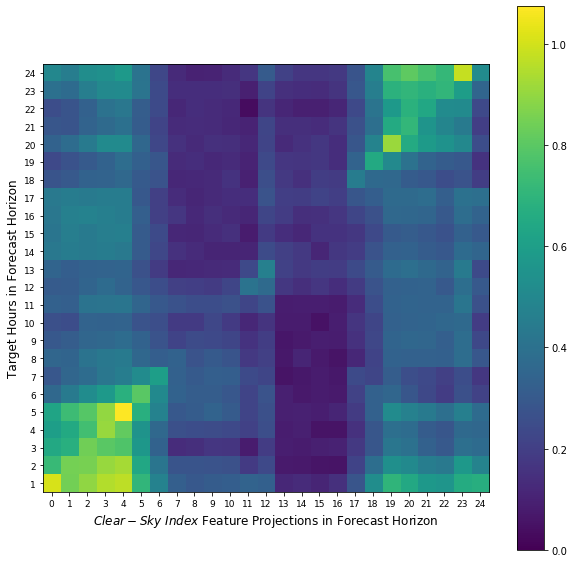
\includegraphics[width=0.65\textwidth]{chapter4/fig_kc_target_mi.png}
    	\caption[Mutual information between Clear-Sky Index feature projections in forecast horizon and irradiance observations for corresponding target hours from fixed-axis solar array]{Mutual information between feature projections of Clear-Sky Index ($K_c$) in the forecast horizon and irradiance observations for corresponding target hours along fixed-axis solar array.}
    	\label{fig:fig_kc_target_mi}
    \end{center}
\end{figure}

\par In Fig.~\ref{fig:fig_kc_target_mi}, it can be seen that the solar irradiance observations are not dependent on all of the $K_c$ feature projections in the forecast horizon. In contrast to the mutual information matrix between the GHI feature projections and solar irradiance observations in the forecast horizon (as in Fig. \ref{fig:fig_ghi_irradiance}), here, the irradiance for a particlar target hour offset in the forecast horizon doesn't necessarily depend on the $K_c$ feature projection corresponding to the same reference time either. As a matter of fact, a lower dependency was observed between the clear-sky index feature projections and target solar irradiance at the center of the forecast horizon.

\par In order to find one such optimal range, a cross-validated grid search was performed. It was identified that the feature projections ranging from 13 hours to 17 hours in the forecast horizon were less relevant. Hence, for the machine learning models trained for each of the target hours, these feature projections were omitted. As a consequence of such an input-selection scheme, 20 feature projections corresponding to clear-sky index and the other NAM weather variables such as air temperature, total cloud cover and height at planetary boundary layer were included as predictors for the machine learning models. Eight temporal encodings (four representing the reference time of the observation, four representing the target hour offset from the reference time) depicting the \textit{time of day} and \textit{time of year} were included as well.

\par Using each of these features as predictors, machine learning models such as \textit{Least-Squares Linear Regression} (LSLR), \textit{k-Nearest Neighbors} (KNN), \textit{Support Vector Regression} (SVR), \textit{Decision Trees} (DT), \textit{Random Forests} (RF) and \textit{Extreme Gradient Boosted Trees} (XGBT) were utilized towards post-processing the solar irradiance from each of the solar arrays. The trivial 24-hour \textit{persistence models} described in Chapter 3 were used as a baseline for this set of experiments as well. For recording the performance of these models, evaluation metrics such as mean absolute error ($MAE$), coefficient of determination ($R^2)$ and Pearson's correlation coefficient ($r$) were used.

\subchapter{Results and Discussion}
\subsubsection*{Assessing Effect of Multi-Model Blending Approaches}
\par In this chapter, the effectiveness of the multi-model blending approaches, i.e. methodologies which combine the NAM Forecast System with the empirical solar radiation models was assessed. Firstly, the performance of the \textit{random forests} algorithm was compared by taking three versions of weather data as input:
\setlist{nolistsep}
\begin{itemize}[noitemsep]
%    \itemsep0em
    \item GHI from NAM Forecast System
    \item adjusted GHI, from blending NAM Forecast System with Clear-Sky Scaling technique \\ (\textit{adjusted} $GHI\textsubscript{NAM+CS}$)
    \item adjusted GHI, from blending NAM Forecast System with Liu-Jordan model \\ (\textit{adjusted} $GHI\textsubscript{NAM+LJ}$)
\end{itemize}

\par In Table \ref{Tab:mmb_array_abe1}, the performance of these predictive models is reported as methodologies \textit{I}, \textit{II} and \textit{III} respectively for each of the dual-axis tracking, fixed-axis and single-axis tracking solar arrays. To enable a smooth comparison with the results reported in chapter 3, and also with the model results from other literature, evaluation metrics such as mean absolute error ($MAE$), coefficient of determination ($R^2$) and Pearson's correlation coefficient ($r$) are reported. The evaluation scheme from Chapter 3, in which the averaged results over 6-hour partitions in the forecast horizon, and the averaged results over the entire forecast horizon is reported, is continued in this chapter too. Both $R^2$ and $r$ over a forecast horizon are computed in a similar fashion as well.
%, by flattening the predictions and ground-truth values for multiple target hours in the forecast horizon into a single array.

\par Random forests utilizing \textit{adjusted} $GHI\textsubscript{NAM+CS}$ performed the best, improving upon those using $GHI\textsubscript{NAM}$ by 4.95\%, 4.53\% and 4.12\% for the dual-axis tracking, fixed axis and single-axis tracking solar arrays respectively. An averaged $MAE$ of 80.61 $W/m^2$, 49.32 $W/m^2$ and 67.52 $W/m^2$ over the entire forecast horizon was reported for each of the solar arrays. An improvement was observed for methodology \textit{III} as well, in which \textit{adjusted} $GHI\textsubscript{NAM+LJ}$ was utilized. Using such a weather forecast dataset resulted in a decrease in $MAE$ by 4.17\%, 4.14\% and 3.62\% respectively, with an $MAE$ of 81.27 $W/m^2$, 49.52 $W/m^2$ and 67.52 $W/m^2$ for the solar arrays.

\vspace{0.6em}

\begin{table}[h]
\begin{center}
    \caption[Evaluating effect of multi-model blending approaches using GHI, on irradiance observations from dual-axis tracking, fixed-axis and single-axis tracking solar arrays, using random forests algorithm.]{Evaluating effect of multi-model blending approaches on irradiance observations from dual-axis tracking, fixed-axis and single-axis tracking solar arrays, using random forests algorithm: \textit{Methodology I} - Using GHI from NAM Forecast System; \textit{Methodology II} - GHI from blending NAM Forecast System and \textit{Clear-Sky Scaling}; \textit{Methodology III} - GHI from blending NAM Forecast System and \textit{Liu-Jordan}.}
    \label{Tab:mmb_array_abe1}
    \begin{tabular}{@{}ccccccccccc@{}}
    \toprule
    \multirow{2}{*}{\textbf{Metric}} & \multirow{2}{*}{\textbf{Horizon}} & \multicolumn{3}{c}{\textbf{Dual-Axis Tracking}} & \multicolumn{3}{c}{\textbf{Fixed-Axis}} & \multicolumn{3}{c}{\textbf{Single-Axis Tracking}}\\
    \cmidrule{3-11}
     &  & \textit{I} & \textit{II} & \textit{III} & \textit{I} & \textit{II} & \textit{III} & \textit{I} & \textit{II} & \textit{III} \\
    
%    \textbf{Metric} & \textbf{Horizon} & \textbf{A} & \textbf{B} & \textbf{C} & \textbf{A} & \textbf{B} & \textbf{C} & \textbf{A} & \textbf{B} & \textbf{C} \\
    \midrule
    \multirow{5}{*}{$MAE$}  & $1 - 6$  & 77.57 & 75.95 & 76.13 & 48.12 & 47.31 & 46.88 & 66.07 & 64.85 & 64.96 \\
           & $6 - 12$       & 86.97 & 83.45 & 83.78 & 52.5  & 51.23 & 51.46 & 72.04 & 69.73 & 69.61 \\
           & $12 - 18$      & 86.62 & 80.43 & 81.05 & 53.13 & 49.42 & 49.89 & 71.04 & 66.1  & 66.79 \\
           & $18 - 24$      & 88.06 & 82.61 & 84.14 & 52.87 & 49.33 & 49.85 & 72.52 & 69.4  & 70.13 \\
           & $Overall$      & 84.81 & \textbf{80.61} & 81.27 & 51.66 & \textbf{49.32} & 49.52 & 70.42 & \textbf{67.52} & 67.87 \\
    \midrule
    \multirow{5}{*}{$R^2$}  & 1 - 6 & 0.86  & 0.86  & 0.86  & 0.91  & 0.91  & 0.91  & 0.87  & 0.87  & 0.87 \\
           & $6 - 12$   & 0.83  & 0.84  & 0.83  & 0.89  & 0.89  & 0.89  & 0.85  & 0.85  & 0.85 \\
           & 12 - 18    & 0.83  & 0.84  & 0.84  & 0.89  & 0.9   & 0.89  & 0.85  & 0.87  & 0.86 \\
           & 18 - 24    & 0.82  & 0.84  & 0.83  & 0.88  & 0.9   & 0.89  & 0.85  & 0.86  & 0.86 \\
           & Overall    & 0.83  & 0.84  & 0.84  & 0.89  & 0.9   & 0.9   & 0.86  & 0.86  & 0.86 \\                     
    \midrule
    \multirow{5}{*}{$r$}  & 1 - 6 & 0.93  & 0.93  & 0.93  & 0.95  & 0.95  & 0.95  & 0.94  & 0.94  & 0.93 \\
           & $6 - 12$   & 0.91  & 0.91  & 0.91  & 0.94  & 0.94  & 0.94  & 0.92  & 0.92  & 0.92 \\
           & 12 - 18    & 0.91  & 0.92  & 0.92  & 0.94  & 0.95  & 0.95  & 0.93  & 0.93  & 0.93 \\
           & 18 - 24    & 0.91  & 0.92  & 0.91  & 0.94  & 0.95  & 0.95  & 0.92  & 0.93  & 0.93 \\
           & Overall    & 0.91  & 0.92  & 0.92  & 0.94  & 0.95  & 0.95  & 0.93  & 0.93  & 0.93 \\                     
    \bottomrule
    \multirow{3}{5em}{Relative Imp. in $MAE$ (\%)} & & & & & & & & & & \\
    & $Overall$ & --- & 4.95\% & 4.17\% & --- & 4.53\% & 4.14\% & --- & 4.12\% & 3.62\% \\ 
    & & & & & & & & & &\\ 
    
    \bottomrule
    \end{tabular}
\end{center}
\end{table}

\par For the next set of experiments, the \textit{random forests} algorithm was combined with the input-selection scheme described in 3.2. This resulted in three versions of input data for the models, in which NAM weather variables such as air temperature, height at planetary boundary layer and total cloud cover were utilized along with the three variants of GHI described earlier. Select feature projections were chosen for each of these meteorological parameters in the predictive models, depending on the target hour offset in the forecast horizon. The results from each of these methodologies is described under \textit{I}, \textit{II} and \textit{III} in Table~\ref{Tab:mmb_array_abe2}.

\par It was observed that both the model-blending approaches observed a slight deterioration in performance. The methodology blending NAM Forecast System with \textit{Clear-Sky Scaling} technique recorded an $MAE$ of 72.57 $W/m^2$, 44.91 $W/m^2$ and 63.56 $W/m^2$ for the dual-axis tracking, fixed-axis and single-axis tracking solar arrays respectively. Meanwhile, combining the NAM Forecast System with Liu-Jordan model recorded an $MAE$ of 72.74 $W/m^2$, 45.25 $W/m^2$ and 63.97 $W/m^2$ for each of the solar arrays.

\begin{table}[h]
\begin{center}
    \caption[Evaluating effect of multi-model blending approaches on irradiance predictions using weather data along dual-axis tracking, fixed-axis and single-axis tracking solar arrays, using random forests algorithm.]{Evaluating effect of multi-model blending approaches on irradiance predictions along dual-axis tracking, fixed-axis and single-axis tracking solar arrays, using random forests algorithm: \textit{Methodology I} - Using input-selected NAM Forecast System; \textit{Methodology II} - Blending input-selected NAM Forecast System and \textit{Clear-Sky Scaling}; \textit{Methodology III} - Blending input-selected NAM Forecast System and \textit{Liu-Jordan}.}
    \label{Tab:mmb_array_abe2}
    \begin{tabular}{@{}ccccccccccc@{}}
    \toprule
    \multirow{2}{*}{\textbf{Metric}} & \multirow{2}{*}{\textbf{Horizon}} & \multicolumn{3}{c}{\textbf{Dual-Axis Tracking}} & \multicolumn{3}{c}{\textbf{Fixed-Axis}} & \multicolumn{3}{c}{\textbf{Single-Axis Tracking}}\\
    \cmidrule{3-11}
     &  & \textit{I} & \textit{II} & \textit{III} & \textit{I} & \textit{II} & \textit{III} & \textit{I} & \textit{II} & \textit{III} \\
    \midrule
     \multirow{5}{*}{$MAE$}  & 1 - 6 & 68.5  & 70.11 & 70.56 & 42.26 & 42.87 & 43.34 & 60.5  & 61.53 & 62.11 \\
           & $6 - 12$   & 72.55 & 72.82 & 73.05 & 45.49 & 45.16 & 45.37 & 63.98 & 63.88 & 64.41 \\
           & 12 - 18    & 70.65 & 72.59 & 72.71 & 44.75 & 45.22 & 45.22 & 62.75 & 63.67 & 63.38 \\
           & 18 - 24    & 74.97 & 74.77 & 74.66 & 46.65 & 46.39 & 47.06 & 66.34 & 65.15 & 65.98 \\
           & Overall    & \textbf{71.67} & 72.57 & 72.74 & \textbf{44.79} & 44.91 & 45.25 & \textbf{63.39} & 63.56 & 63.97 \\                     

    \midrule
    \multirow{5}{*}{$R^2$}  & 1 - 6 & 0.88  & 0.88  & 0.88  & 0.92  & 0.92  & 0.92  & 0.89  & 0.89  & 0.89 \\
           & $6 - 12$   & 0.87  & 0.87  & 0.87  & 0.91  & 0.91  & 0.91  & 0.87  & 0.87  & 0.87 \\
           & 12 - 18    & 0.87  & 0.87  & 0.87  & 0.91  & 0.91  & 0.91  & 0.88  & 0.88  & 0.88 \\
           & 18 - 24    & 0.86  & 0.86  & 0.86  & 0.9   & 0.91  & 0.9   & 0.87  & 0.87  & 0.87 \\
           & Overall    & 0.87  & 0.87  & 0.87  & 0.91  & 0.91  & 0.91  & 0.88  & 0.88  & 0.88 \\                     
    \midrule
    \multirow{5}{*}{$r$}  & 1 - 6 & 0.94  & 0.94  & 0.94  & 0.96  & 0.96  & 0.96  & 0.94  & 0.94  & 0.94 \\
           & $6 - 12$   & 0.93  & 0.93  & 0.93  & 0.95  & 0.96  & 0.95  & 0.93  & 0.93  & 0.93 \\
           & 12 - 18    & 0.93  & 0.93  & 0.93  & 0.95  & 0.96  & 0.96  & 0.94  & 0.94  & 0.94 \\
           & 18 - 24    & 0.93  & 0.93  & 0.93  & 0.95  & 0.95  & 0.95  & 0.93  & 0.93  & 0.93 \\
           & Overall    & 0.93  & 0.93  & 0.93  & 0.95  & 0.96  & 0.96  & 0.94  & 0.94  & 0.94 \\                     

    \bottomrule
    \end{tabular}
\end{center}
\end{table}

\par In general, the addition of weather variables has shown to incorporate site-specific information into the predictive models. In Chapter 3, the selective picking of feature projections of NAM weather variables in the forecast horizon improved the performance of the predictive models considerably. A similar improvement in performance was expected by including additional weather data with the model-blended GHI as well. However, this wasn't the case. This can possibly be attributed to the misidentification of clear-sky conditions by clear-sky index and clearness index respectively. Such a misidentification could have led to an adjustment in GHI, where it wasn't needed.

\subsubsection*{Performance Evaluation for Predictive Modeling using Clear-Sky Index}
\par In this series of experiments, meteorological variables including relevant NAM weather variables and clear-sky index was utilized. The machine learning models were trained on such weather data corresponding to 2017, and evaluated against that corresponding to 2018. For the dual-axis tracking solar array, all the models performed better than the baseline $t-24$ persistence models, which was expected. \textit{Random forests} performed the best, recording an $MAE$ of 79.58 $W/m^2$. However, this was worse in comparison to the performance of this model utilizing input-selected NAM forecast data (as in Table~\ref{Tab:fs_array_a}), for which an $MAE$ of 72.63 $W/m^2$ was observed. In addition, a considerable degradation in performance was observed in the performance of \textit{support vector regression}, the $MAE$ of which increased from 73.43 $W/m^2$ to 83.2 $W/m^2$, and for \textit{k-nearest neighbors}, whose $MAE$ increased from 73.02 $W/m^2$ to 98.52 $W/m^2$.

\begin{table}[h]
\begin{center}
    \caption{Evaluating performance of predictive models using Clear-Sky Index, for irradiance predictions along dual-axis tracking solar array.}
    \vspace{0.2cm}
    \label{Tab:mmb_array_a}
    \begin{tabular}{ccccccccc}
    \toprule
    \textbf{Metric} & \textbf{Horizon} & \textbf{PER} & \textbf{LSLR} & \textbf{SVR} & \textbf{KNN} & \textbf{DT} & \textbf{RF} & \textbf{XGBT} \\
    \midrule
    \multirow{5}{*}{$MAE$}  & $1 - 6$ & 153.32 & 119.41 & 80.21 & 99.59  & 75.96 & 78.52 & 78.52 \\
                            & $7 - 12$ & 153.91 & 134.82 & 82.3  & 94.59  & 79.9  & 77.8  & 79.98 \\
                            & $13 - 18$ & 154.16 & 118.45 & 84.08 & 98.35  & 82.29 & 80.44 & 80.63 \\
                            & $19 - 24$ & 161.43 & 134.98 & 86.19 & 101.54 & 83.76 & 81.55 & 81.36 \\
                            & $Overall$ & 155.71 & 126.92 & 83.2  & 98.52  & 80.48 & \textbf{79.58} & 80.12 \\
                            \midrule
    \multirow{5}{*}{$R^2$}  & $1 - 6$ & 0.46 & 0.82   & 0.87  & 0.71   & 0.86  & 0.86  & 0.86  \\
                            & $7 - 12$ & 0.45 & 0.78   & 0.86  & 0.74   & 0.85  & 0.86  & 0.85  \\
                            & $13 - 18$ & 0.45 & 0.82   & 0.86  & 0.72   & 0.84  & 0.85  & 0.85  \\
                            & $19 - 24$ & 0.41 & 0.76   & 0.84  & 0.71   & 0.84  & 0.85  & 0.85  \\
                            & $Overall$ & 0.44 & 0.79   & 0.85  & 0.72   & 0.85  & 0.85  & 0.85  \\
                            \midrule
    \multirow{5}{*}{$r$}    & $1 - 6$ & 0.73 & 0.91   & 0.93  & 0.86   & 0.93  & 0.93  & 0.93  \\
                            & $7 - 12$ & 0.73 & 0.88   & 0.93  & 0.87   & 0.92  & 0.93  & 0.92  \\
                            & $13 - 18$ & 0.73 & 0.91   & 0.93  & 0.86   & 0.92  & 0.92  & 0.92  \\
                            & $19 - 24$ & 0.71 & 0.87   & 0.92  & 0.85   & 0.91  & 0.92  & 0.92  \\
                            & $Overall$ & 0.72 & 0.89   & 0.93  & 0.86   & 0.92  & 0.93  & 0.92 \\    
    \bottomrule
    \end{tabular}
\end{center}
\end{table}

\par \textit{k-Nearest Neighbors} algorithm does not make any assumptions about the distribution of the data. In this methodology, the feature projections corresponding to GHI are replaced with those of clear-sky index, which have a lesser bias and variance as compared to the former. Thus, a more rigorous cross-validated grid search can be performed to find a better set of hyperparameters. Doing so  might improve the model complexity and help in attaining a better model fit. 

\par The decrease in performance of \textit{support vector regression} can posssibly be attributed to the $C$ hyperparameter, which represents the strength of regularization. With the change in data distribution due to the substitution of GHI feature projections with those corresponding to clear-sky index, the decrease in bias should be compensated with an increase in $C$. Doing so would decrease the regularization penalty on the predictive models, and might improve the performance. This was not accounted for during the training of the predictive models using clear-sky index.

\begin{table}[h]
\begin{center}
    \caption{Evaluating performance of predictive models using Clear-Sky Index, for irradiance predictions along fixed-axis solar array.}
    \vspace{0.2cm}
    \label{Tab:mmb_array_b}
%    \begin{tabular}{@{}p{5.3em}cccccccc@{}}
    \begin{tabular}{ccccccccc}
    \toprule
    \textbf{Metric} & \textbf{Horizon} & \textbf{PER} & \textbf{LSLR} & \textbf{SVR} & \textbf{KNN} & \textbf{DT} & \textbf{RF} & \textbf{XGBT} \\ 
    \midrule
    \multirow{5}{*}{$MAE$} & $1 - 6$ & 111.23 & 76.68 & 50.51 & 59.50  & 48.07 & 48.25 & 50.62 \\
                             & $7 - 12$ & 111.51 & 84.61 & 52.89 & 60.35 & 52.34 & 47.76 & 51.36 \\
                             & $13 - 18$ & 111.97 & 81.33 & 54.87 & 64.85 & 53.68 & 49.55 & 50.92 \\
                             & $19 - 24$ & 117.15 & 88.48 & 56.06 & 63.35 & 53.55 & 51.17 & 51.87 \\
                             & $Overall$ & 112.96 & 82.77 & 53.58 & 62.01 & 51.91 & \textbf{49.18} & 51.20 \\
    \midrule
    \multirow{5}{*}{$R^2$} & $1 - 6$ & 0.59 & 0.88  & 0.91  & 0.83  & 0.90 & 0.91 & 0.90 \\
                             & $7 - 12$ & 0.58 & 0.86  & 0.90   & 0.82  & 0.89  & 0.90 & 0.89 \\
                             & $13 - 18$ & 0.58 & 0.87  & 0.90   & 0.80   & 0.89  & 0.90 & 0.90 \\
                             & $19 - 24$ & 0.55 & 0.83  & 0.88  & 0.81  & 0.88  & 0.90 & 0.89 \\
                             & $Overall$ & 0.58 & 0.86  & 0.90   & 0.81  & 0.89  & 0.90 & 0.90 \\ 
    \midrule
    \multirow{5}{*}{$r$}    & $1 - 6$ & 0.79 & 0.94  & 0.96  & 0.91 & 0.95  & 0.96 & 0.95  \\
                            & $7 - 12$ & 0.79 & 0.93  & 0.95  & 0.91 & 0.95  & 0.95 & 0.95  \\
                            & $13 - 18$ & 0.79 & 0.93  & 0.95  & 0.90 & 0.94  & 0.95 & 0.95  \\
                            & $19 - 24$ & 0.78 & 0.91  & 0.94  & 0.90 & 0.94  & 0.95 & 0.95  \\
                            & $Overall$ & 0.79 & 0.93  & 0.95  & 0.90 & 0.94  & 0.95 & 0.95  \\
    \bottomrule
    \end{tabular}
\end{center}
\end{table}

\par Similar trends were observed for the predictions along fixed-axis and single-axis tracking solar arrays as well. \textit{Random forests} performed the best, recording an $MAE$ of 49.18 $W/m^2$ and 69.98 $W/m^2$ respectively for each of the solar arrays. This performance was worse when compared with the best accuracy obtained by machine learning models utilizing input-selected NAM weather dataset (as in Table~\ref{Tab:fs_array_b} and Table~\ref{Tab:fs_array_e}). There, an $MAE$ of 44.94 $W/m^2$ and 63.60 $W/m^2$ was recorded for both the solar arrays respectively. Though the overall performance of predictive models using clear-sky index worsened, in order to examine the cyclicity-capturing ability of these models, a stratified diurnal and seasonal analysis of the performance of the predictive models with respect to target irradiance predictions on the fixed-axis solar array is performed. 

\begin{table}[h]
\begin{center}
    \caption{Evaluating performance of predictive models using Clear-Sky Index, for irradiance predictions along single-axis tracking solar array.}
    \vspace{0.2cm}
    \label{Tab:mmb_array_e}
    \begin{tabular}{ccccccccc}
    \toprule
    \textbf{Metric} & \textbf{Horizon} & \textbf{PER} & \textbf{LSLR} & \textbf{SVR} & \textbf{KNN} & \textbf{DT} & \textbf{RF} & \textbf{XGBT} \\
    \midrule
    \multirow{5}{*}{$MAE$} & $1 - 6$ & 128.64 & 94.40   & 68.81 & 85.56 & 68.16 & 69.6 & 70.55 \\
                             & $7 - 12$ & 128.97 & 107.51 & 72.16 & 81.62 & 72.58 & 68.46 & 69.09 \\
                             & $13 - 18$ & 129.25 & 98.92  & 72.48 & 87.56 & 72.49 & 69.39 & 69.50 \\
                             & $19 - 24$ & 135.35 & 102.31 & 73.88 & 86.56 & 74.25 & 72.45 & 72.84\\
                             & $Overall$ & 130.55 & 100.78 & 71.83 & 85.33 & 71.87 & \textbf{69.98} & 70.50 \\ 
    \midrule
    \multirow{5}{*}{$R^2$} & $1 - 6$ & 0.53 & 0.85   & 0.87  & 0.75  & 0.86  & 0.87 & 0.86 \\
                             & $7 - 12$ & 0.53 & 0.81   & 0.86  & 0.77  & 0.85  & 0.86 & 0.86 \\
                             & $13 - 18$ & 0.53 & 0.84   & 0.86  & 0.74  & 0.85  & 0.86 & 0.86 \\
                             & $19 - 24$ & 0.49 & 0.83   & 0.86  & 0.75  & 0.85  & 0.86 & 0.86 \\ 
                             & $Overall$ & 0.52 & 0.82   & 0.85  & 0.74  & 0.84  & 0.85 & 0.85 \\
    \midrule
    \multirow{5}{*}{$r$}    & $1 - 6$ & 0.77 & 0.92 & 0.94  & 0.88  & 0.93  & 0.93 & 0.93  \\
                            & $7 - 12$ & 0.77 & 0.90 & 0.93  & 0.89  & 0.92  & 0.93 & 0.92  \\
                            & $13 - 18$ & 0.75 & 0.92 & 0.93  & 0.87  & 0.92  & 0.93 & 0.93  \\
                            & $19 - 24$ & 0.75 & 0.91 & 0.92  & 0.87  & 0.92  & 0.92 & 0.92  \\
                            & $Overall$ & 0.76 & 0.91 & 0.93  & 0.87  & 0.92  & 0.93 & 0.93   \\
    \bottomrule
    \end{tabular}
\end{center}
\end{table}

\subsubsection*{Stratified Diurnal and Seasonal Analysis of Performance}

\par The stratified diurnal analysis conducted in Chapter 3 was extended to the predictive models utilizing clear-sky index as well. In Fig.~\ref{fig:fig_stratified_diurnal_kc}, the performance of the machine learning models for all target hours in the forecast horizon, were plotted for each of the 00h, 06h, 12h and 18h UTC NAM forecasts individually. The time of day was presumed to be between 6 A.M and 6 P.M at the target location, and was highlighted in yellow. In general, as was expected, it was observed that most of the models were able to detect the period of darkness, i.e. night-time relatively well.

\begin{figure}[ht]
    \begin{center}
    	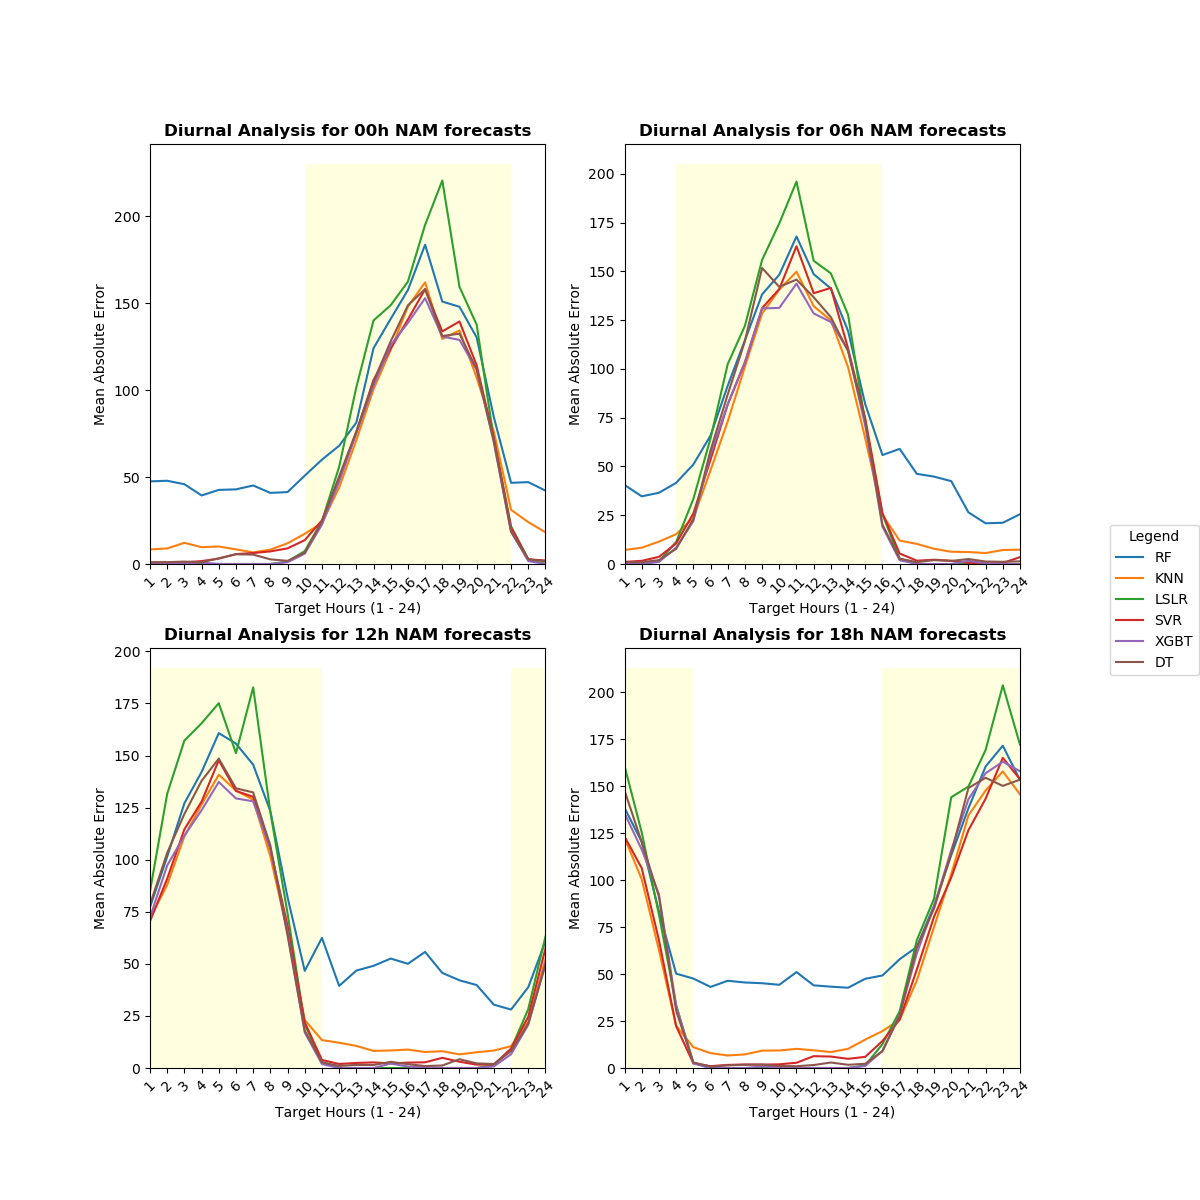
\includegraphics[width=0.9\textwidth, height=12cm]{chapter4/fig_diurnal_arrayb.png}
    	\caption[Stratified diurnal analysis of day-ahead irradiance predictions using Clear-Sky Index for fixed-axis solar array]{Stratified diurnal analysis of day-ahead irradiance predictions using Clear-Sky Index for fixed-axis solar array: (left-top) 00h NAM forecasts, (right-top) 16h NAM forecasts, (left-bottom) 12h NAM forecasts, (right-bottom) 18h NAM forecasts. Local time of day (6A.M to 6P.M) at the target location for each of the NAM forecasts is indicated in light yellow.}
    	\label{fig:fig_stratified_diurnal_kc}
    \end{center}
\end{figure}


\par For the period of day, the more sophisticated machine learning algorithms like \textit{k-nearest neighbors}, \textit{support vector regression} and \textit{random forests} performed better than \textit{decision trees}, and understandably, \textit{linear regression}. However, interestingly enough, \textit{extreme gradient boosted trees} failed to capture day-time well for all the NAM forecasts. This can possibly be attributed to a lesser number of decision trees being used in the ensemble technique. In addition, the diurnal performance of the best performing \textit{random forests} with respect to its performance when utilizing the input-selected NAM weather forecast data (as shown in Fig.~\ref{fig:fig_stratified_diurnal}) can be summarized in the following way:
\setlist{nolistsep}
\begin{itemize}[noitemsep]
    \item performed worse for all the target hours in the day-time for the 00h NAM forecasts
    \item performed better for the target hours 8 through 12 in the forecast horizon, for the 06h NAM forecasts
    \item performed better for the target hours 22 through 24 in the forecast horizon, for the 12h NAM forecasts
    \item performed worse for all the target hours in the day-time for the 18h NAM forecasts
\end{itemize}

\par The target location, i.e. Athens, Georgia is -5.00 hours with respect to UTC in the standard time zone, and -4.00 hours with respect to UTC during \textit{daylight saving time}. To be able to conduct a uniform analysis of the individual NAM forecasts, it was assumed that the local time at the target location is constantly -4.00 hours relative to UTC. 

\par Based on this assumption, as was done in Chapter 3, the performance of different predictive models was compared by analyzing their residuals corresponding to the target hour in the forecast horizon, representing noon, i.e. 12 P.M locally at Athens, Georgia. In Fig.~\ref{fig:fig_noon_whisker}, box-and-whisker plots were drawn corresponding to the residuals from each of the predictive models, so as to study their distributional characteristics. In the figure, the size of the box-plots for most of the models is comparable. In addition, the spread of the residuals beyond the whiskers is minimum for \textit{random forests}, indicating that it is the better machine learning technique for this variant of weather data.

\begin{figure}[ht]
    \begin{center}
%    	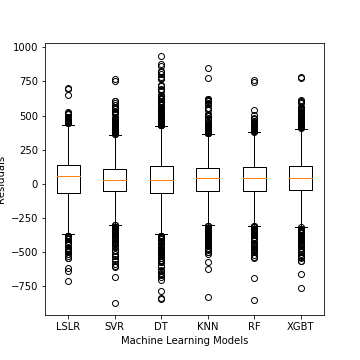
\includegraphics[width=0.75\textwidth, height=8cm]{chapter4/fig_whiskers_csi.png}
    	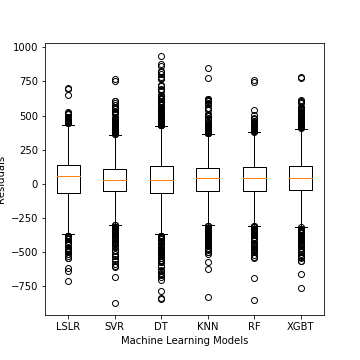
\includegraphics[scale=0.75]{chapter4/fig_whiskers_csi.png}
    	\caption[Comparison of box-and-whisker plots of residuals from different predictive models utilizing clear-sky index at 12 P.M local time]{Comparison of box-and-whisker plots of residuals from different predictive models utilizing clear-sky index at 12 P.M local time, i.e. noon.}
    	\label{fig:fig_noon_whisker}
    \end{center}
\end{figure}

\par Furthermore, a stratified seasonal analysis was conducted for NAM forecasts. It was extended to the 12h and 18h NAM forecasts, which, under the above assumption, represent 8 A.M and 12 P.M locally. Based on the general seasonal trends in the target location i.e. Athens, Georgia, the periods in a year were divided into four seasons: \textit{summer} (May - July), \textit{autumn} (August - October), \textit{winter} (November - January) and \textit{spring} (February - April).

\begin{table}[htbp]
\begin{center}
\caption[Comparing seasonal performance of random forests using input-selected NAM data with GHI and Clear-Sky Index for 12h, 18h NAM forecasts]{Comparing seasonal performance (in $MAE$) of random forests using input-selected NAM data with GHI (left) and clear-sky index (right) for 12h, 18h NAM forecasts.}
\label{tab:seasonal_comparison}
\begin{tabular}{cccccc}
\toprule
\multirow{2}{*}{\textbf{Model}} & \multirow{2}{*}{\textbf{Hour}} & \multicolumn{4}{c}{\textbf{NAM using GHI} / \textbf{NAM using Clear-Sky Index}}   \\ \cmidrule{3-6} 
& & \textit{Summer} & \textit{Autumn} & \textit{Winter} & \textit{Spring} \\
\midrule
LSLR           & 12h                    & 60.21 / 67.41           & 86.35 / 106.9           & 99.71 / 121.9           & 119.4 / 138.1 \\
               & 18h                    & 84.93 / 112.9          & 95.13 / 121.0           & 70.82 / 91.61           & 38.68 / 49.09 \\
SVR            & 12h                    & 46.95 / 64.11          & 64.01 / 74.95           & 72.02 / 88.05           & 84.52 / 102.6   \\
               & 18h                    & 76.11 / 102.4           & 78.75 / 94.32           & 49.03 / 60.49           & 12.39 / 19.49 \\
DT             & 12h                    & 74.60 / 90.51           & 104.4 / 107.9          & 101.8 / 116.4          & 128.3 / 171.6 \\
               & 18h                    & 110.8 / 127.7          & 109.2 / 124.8           & 57.45 / 85.56           & 24.34 / 36.59 \\
KNN            & 12h                    & 54.16 / 58.54          & 81.13 / 83.87           & 89.93 / 90.19           & 98.44 / 87.89 \\
               & 18h                    & 87.39 / 102.5          & 87.52 / 102.4          & 62.32 / 74.12           & 16.25 / 18.76 \\
RF             & 12h                    & 56.15 / 75.93           & 82.91 / 101.9          & 95.77 / 114.0          & 107.5 / 123.0 \\
               & 18h                    & 80.52 / 139.3           & 81.73 / 119.8           & 56.84 / 94.25          & 10.47 / 29.03 \\
XGBT           & 12h                    & 54.07 / 74.41          & 86.37 / 98.35           & 101.1 / 123.3          & 119.2 / 126.0 \\
               & 18h                    & 80.66 / 134.9          & 85.68 / 128.1           & 56.24 / 96.10          & 10.50 / 27.75 \\ \bottomrule
\end{tabular}
\end{center}
\end{table}

\par In Table~\ref{tab:seasonal_comparison}, the performance of the better-performing \textit{random forests} across each of these seasons was compared. The $MAE$ corresponding to predictions of the models utilizing NAM data involving both GHI and clear-sky index was included. It can be observed that the predictive models using clear-sky index performed poorly for both the 12h and 18h NAM forecasts across all the seasons. Moreover, as was noted earlier in the diurnal analysis, the 18h NAM forecasts performed poorly for all the target hours in the forecast horizon. Owing to the relatively poor performance of the NAM forecasts involving clear-sky index, as against those involving GHI, it can be concluded that using the clear-sky index as a predictor in the machine learning models failed to improve the diurnal and seasonal trend capturing ability of the models.



\newpage